% !TeX program = pdflatex
% !TeX root = ../main.tex

%*******************************************************
% Ringraziamenti
%*******************************************************
\cleardoublepage
\phantomsection
\pdfbookmark{Acknowledgments}{acknowledgments}

\chapter*{Acknowledgments}
\markboth{\spacedlowsmallcaps{Acknowledgments}}%
	{\spacedlowsmallcaps{Acknowledgments}}
\thispagestyle{empty}

%\vspace*{-20pt}

%\begin{flushright}{\slshape    
%	Lorem ipsum dolor sit amet, consectetuer adipiscing elit. \\
%	Ut purus elit, vestibulum ut, placerat ac, adipiscing vitae, felis. \\
%	Curabitur dictum gravida mauris.} \\ \medskip
%    --- Donald Ervin Knuth
%\end{flushright}

\vspace{5pt}

I started my PhD student experience with a suboptimal attitude, since personal
and referred experiences made me rather critical about academia as a whole, and
I despised some of the dynamics \textit{naturally} associated with the research
environment, which many had the \textit{pleasure} to experience.

Nevertheless, I have been extremely lucky: lucky from the very beginning, since
even before starting I got some kind advice from members of the institution
where I was a student, that have done their best to motivate me and to show
some interesting directions worth to investigate.
For this, I am grateful to professors Enrico Trincherini and Gigi Rolandi, and
my master thesis advisor Massimo D'Elia. 
It is extremely likely that without them, I would have not even started the PhD
adventure.

Yet the beginning of a significant journey is always very far from its end, and
I considered many times if just keep going would have been a somewhat optimal
choice. There is no such a thing as a straight way, and there has been many
non-trivial steps in my own, I got to the end through all the choices done.
%
For this, it has been fundamental not to be alone. I shared this experience
with several of my friends from Pisa, that accompanied me for the five years of
our Bachelor and Master. Their example and more direct discussions closed the
geographical gap between us.
Among them, I should thank in particular Marco Costa, since he strongly
supported me, in particular at the very beginning.
%
But even more, I should thank the members of our Milan group, in the order I
met them: Juan Cruz-Martinez, Christopher Schwan, Tanjona Rabemananjara, and
Roy Stegeman, since working with them have been many times the strongest
motivation to dedicate my entire self to our common goals.
A separate mention has to be dedicated to Felix Hekhorn, since he assisted me
while still learning the job almost from zero, and we kept working together
every day: literally every day and all day long during the times of the global
pandemic. I have never been feeling really isolated, and in practice this is
mostly due to him, that lead me and had the patience to teach me everything.
Even if they arrived later on, also Giacomo Magni, Andrea Barontini, and
Niccol\`o Laurenti have been optimal companions to share a relevant part of the
journey.

It is sometimes a trivial addition to this list the presence of each one's
supervisor. I am not going to disobey this consolidated tradition, but I would
like to remark how non-trivial this is for me.
As already mentioned, even before starting I have been aware of many negative
experiences. But this has not been my case, entirely thanks to prof. Stefano
Forte.
%
He has been welcoming from the very first day, when I met him in Milan without
even knowing I were looking for a PhD position.
His door was every day open to my questions, to solve my doubts and discuss my
proposals. He never just dismissed any issue, and carefully listened also to my
personal concerns, encouraging me to continue this career.

It has also been incredibly formative to work in the \nnpdf collaboration lead
by him, and to see various problems arising from working as a group, together
with many solutions.
It is definitely a complex task to coordinate with each other, but it is the
only way to achieve certain results.
This entire thesis gather many contributions from \nnpdf members, and I am
really thankful to all of them. Not only thankful for the work done together,
but also for the many lessons I learnt in the process.
It took time, but I appreciated different virtues of each one. Diversity is
essential for any complex task, and it is completely lost if limiting ourselves
to work alone.

Finally, my greatest gratitude goes to my family, in particular my parents,
Paolo and Lucia.
It might seem like they have done nothing for my PhD, but if I have been able
to work on it, it has been thanks to their every day support, both from the
practical and emotional point of view.
%
In a very similar way I am grateful to my partner, Viviana. But I owe her
something more: she decided to move together with me from Pisa to Milan, to
start together a new journey, and to live together every day.
She encouraged and supported me so many times and in so many ways.
%
During my education I have been taught to often remind that
\textit{\enquote{non di solo pane vive l'uomo}}, and definitely research on its
own is not enough for me.

\bigskip
\bigskip
 
\noindent\textit{\myLocation, \MakeTextLowercase{\myTime}}

\smallskip
\vspace*{-20pt}

\begin{flushright}
	\begin{tabular}{m{5cm}}
		\\ \hline
		\centering\myName \\
	\end{tabular}
\end{flushright}

\vfill

\pagebreak

\vfill

\begin{figure}
	\centering
	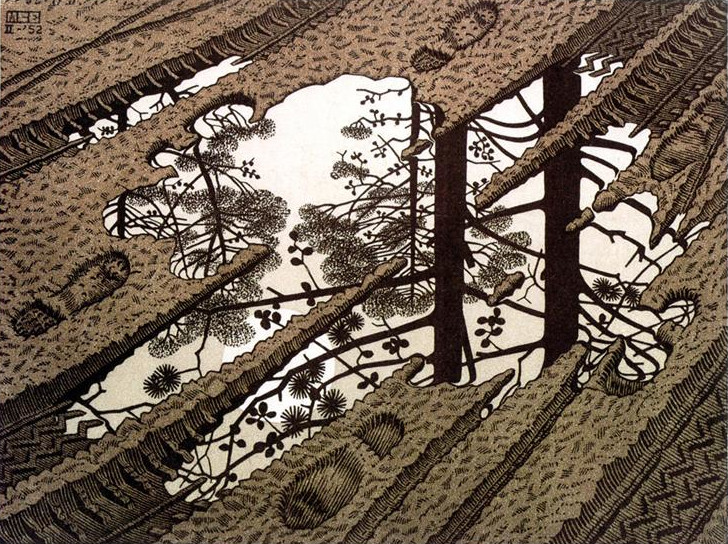
\includegraphics[width=0.9\textwidth]{puddle}
\end{figure}

\vfill
